\documentclass[aspectratio=169,11pt,hyperref={colorlinks=true}]{beamer}
% https://github.com/zr-tex8r/BXcjkjatype/blob/master/README-ja.md
\usepackage[whole]{bxcjkjatype}
\usetheme{boxes}
\setbeamertemplate{navigation symbols}{}
\definecolor{suse}{RGB}{2, 211, 95}
\definecolor{susedark}{RGB}{13, 44, 64}
\setbeamercolor{titlelike}{fg=suse}
\setbeamercolor{structure}{fg=suse}
\hypersetup{colorlinks,urlcolor=suse}
\setbeamertemplate{footline}[frame number]
% Inserting graphics
\usepackage{graphicx}
% Side-by-side figures, etc
\usepackage{subfigure}
% Code snippits
\usepackage{listings}
% Color stuff
\usepackage{color}
% underline
\usepackage{soul}

\usepackage{amsmath}
\usepackage{tikz}
\newcommand\RBox[1]{%
  \tikz\node[draw,rounded corners,align=center,] {#1};%
}
\usepackage{hyperref}
%\usecolortheme{buzz}
%\usecolortheme{wolverine}
%\usetheme{Boadilla}
\usepackage[T1]{fontenc}
%\usepackage{fontspec}
%\usepackage[expert, deluxe]{otf}

\definecolor{mygreen}{rgb}{0,0.6,0}
\definecolor{mygray}{rgb}{0.5,0.5,0.5}
\definecolor{mymauve}{rgb}{0.58,0,0.82}


%\usepackage{CJK}
%\pdfmapline{=genshingothic@Unicode@ <genshingothic.ttf}
% bxcjkjatype
%\setgothicfont[<ID>]{<フォントファイル名>}
%\setgothicfont{/Users/foo/Library/Fonts/genshingothic.ttf}
%\setgothicfont{/Users/foo/Library/Fonts/NotoSansCJKjp-Regular.otf}
%\setgothicfont{/Users/foo/Downloads/genshingothic-20150607/GenShinGothic-P-Normal.ttf}
%\setgothicfont{/Users/foo/Downloads/genshingothic-20150607/GenShinGothic-Regular.ttf}
%\setgothicfont{hiragino.ttc}
\setgothicfont{mplus-1p-regular.ttf}
\setCJKfamilydefault{\gtdefault}
%\setCJKfamilydefault{\mcdefault}
%\CJKforce{abcdefghijklmnopqrstuvwxyzABCDEFGHIJKLMNOPQRSTUVWXYZ}


\lstset{%
  backgroundcolor=\color{susedark},   % choose the background color; you must add \usepackage{color} or \usepackage{xcolor}
  breakatwhitespace=false,         % sets if automatic breaks should only happen at whitespace
  breaklines=true,                 % sets automatic line breaking
  captionpos=b,                    % sets the caption-position to bottom
  commentstyle=\color{suse},  % comment style
  extendedchars=true,              % lets you use non-ASCII characters; for 8-bits encodings only, does not work with UTF-8
  keepspaces=true,                 % keeps spaces in text, useful for keeping indentation of code (possibly needs columns=flexible)
  keywordstyle=\color{blue},       % keyword style
%  otherkeywords={*,...},           % if you want to add more keywords to the set
  numbersep=5pt,                   % how far the line-numbers are from the code
  numberstyle=\tiny\color{mygray}, % the style that is used for the line-numbers
  rulecolor=\color{white},         % if not set, the frame-color may be changed on line-breaks within not-black text (e.g. comments (green here))
  showspaces=false,                % show spaces everywhere adding particular underscores; it overrides 'showstringspaces'
  showstringspaces=false,          % underline spaces within strings only
  showtabs=false,                  % show tabs within strings adding particular underscores
  stringstyle=\color{suse},   % string literal style
}

\setbeamerfont{caption}{series=\normalfont,size=\fontsize{6}{8}}
%\setbeamerfont{caption}{series=\normalfont,size=\large}
\setbeamertemplate{caption}{\raggedright\insertcaption\par}

\setlength{\abovecaptionskip}{0pt}
\setlength{\floatsep}{0pt}

\author[Masayuki Igawa]{%
  \texorpdfstring{%
    \centering
    Masayuki Igawa\\
    \href{mailto:masayuki@igawa.io}{masayuki@igawa.io}\\
    \texttt{masayukig on \href{http://freenode.net/}{Freenode},
     \href{https://twitter.com/masayukig}{Twitter},
     \href{https://github.com/masayukig}{GitHub}}
  }
  {Masayuki Igawa}
}
\date{May 30, 2017}
\def\place#1{\def\@place{#1}}
\place{\href{https://mesos.connpass.com/event/57331/}{@Mesos Meetup Tokyo \#1}}

\title[Mesos, DC/OS on openSUSE
\hspace{2em}\insertframenumber/\inserttotalframenumber]{Mesos, DC/OS on openSUSE}

\setbeamercolor{background canvas}{bg=susedark}
\setbeamercolor{titlelike}{fg=white}
\setbeamercolor{structure}{fg=white}
\setbeamercolor{normal text}{fg=white}
\begin{document}

{%
% \setbeamertemplate{background canvas}{
\includegraphics[width=\paperwidth,height=\paperheight]{background_title.png}}
\setbeamertemplate{footline}{}
\setbeamercolor{background canvas}{bg=susedark}
\begin{frame}[noframenumbering]
  \hypersetup{colorlinks,urlcolor=suse}
  \setbeamercolor{author}{fg=white}
  \setbeamercolor{date}{fg=white}
  \setbeamercolor{place}{fg=white}
  \titlepage{}
  \centering
  \@place \par
  \href{https://github.com/masayukig/mesos-dcos-on-opensuse}{github.com/masayukig/mesos-dcos-on-opensuse}
\end{frame}
}

% \section{Agenda}
% \begin{frame}
%   \frametitle{Agenda}
%   \begin{itemize}
%     \item 自己紹介
%     \item やりたいこと
%     \item やってみた
%     \item どうなった?(困ったこと)
%     \item 解決方法
%     \item まとめ
%   \end{itemize}
% \end{frame}

\section{Introduction}
\begin{frame}
  \frametitle{自己紹介}
  \begin{columns}[T]
    \begin{column}{.5\textwidth}
      \begin{itemize}
        \item 所属企業:SUSE/ノベル株式会社
          \begin{itemize}
            \item QE(Quality Engineering)チーム所属
            \item[] (日本にいるのは私だけ)
            \item \href{https://www.suse.com/newsroom/post/2016/suse-acquires-openstack-iaas-and-cloud-foundry-paas-talent-and-technology-assets-from-hpe-to-accelerate-growth-and-entry-into-new-markets/}{SUSE Acquires OpenStack IaaS and Cloud Foundry PaaS Talent and Technology Assets from HPE to Accelerate Growth and Entry into New Markets}
          \end{itemize}
        \item 業務: オープンソースプログラマ
          \begin{itemize}
            \item \href{https://www.openstack.org/}{OpenStack}
             \href{https://wiki.openstack.org/wiki/QA}{QA} 領域でアップストリームを通じた開発:
             \href{https://docs.openstack.org/developer/tempest/}{Tempest},
             \href{http://status.openstack.org/openstack-health/}{OpenStack-Health},
             \href{https://docs.openstack.org/developer/subunit2sql/}{Subunit2SQL},
             \href{https://docs.openstack.org/developer/stackviz/}{Stackviz}等のコアレビューア
            \item \href{http://stackalytics.com/?user_id=igawa&release=all&metric=all}{stackalytics.com/?user\_id=igawa}
          \end{itemize}
      \end{itemize}
    \end{column}
    \begin{column}{.5\textwidth}
      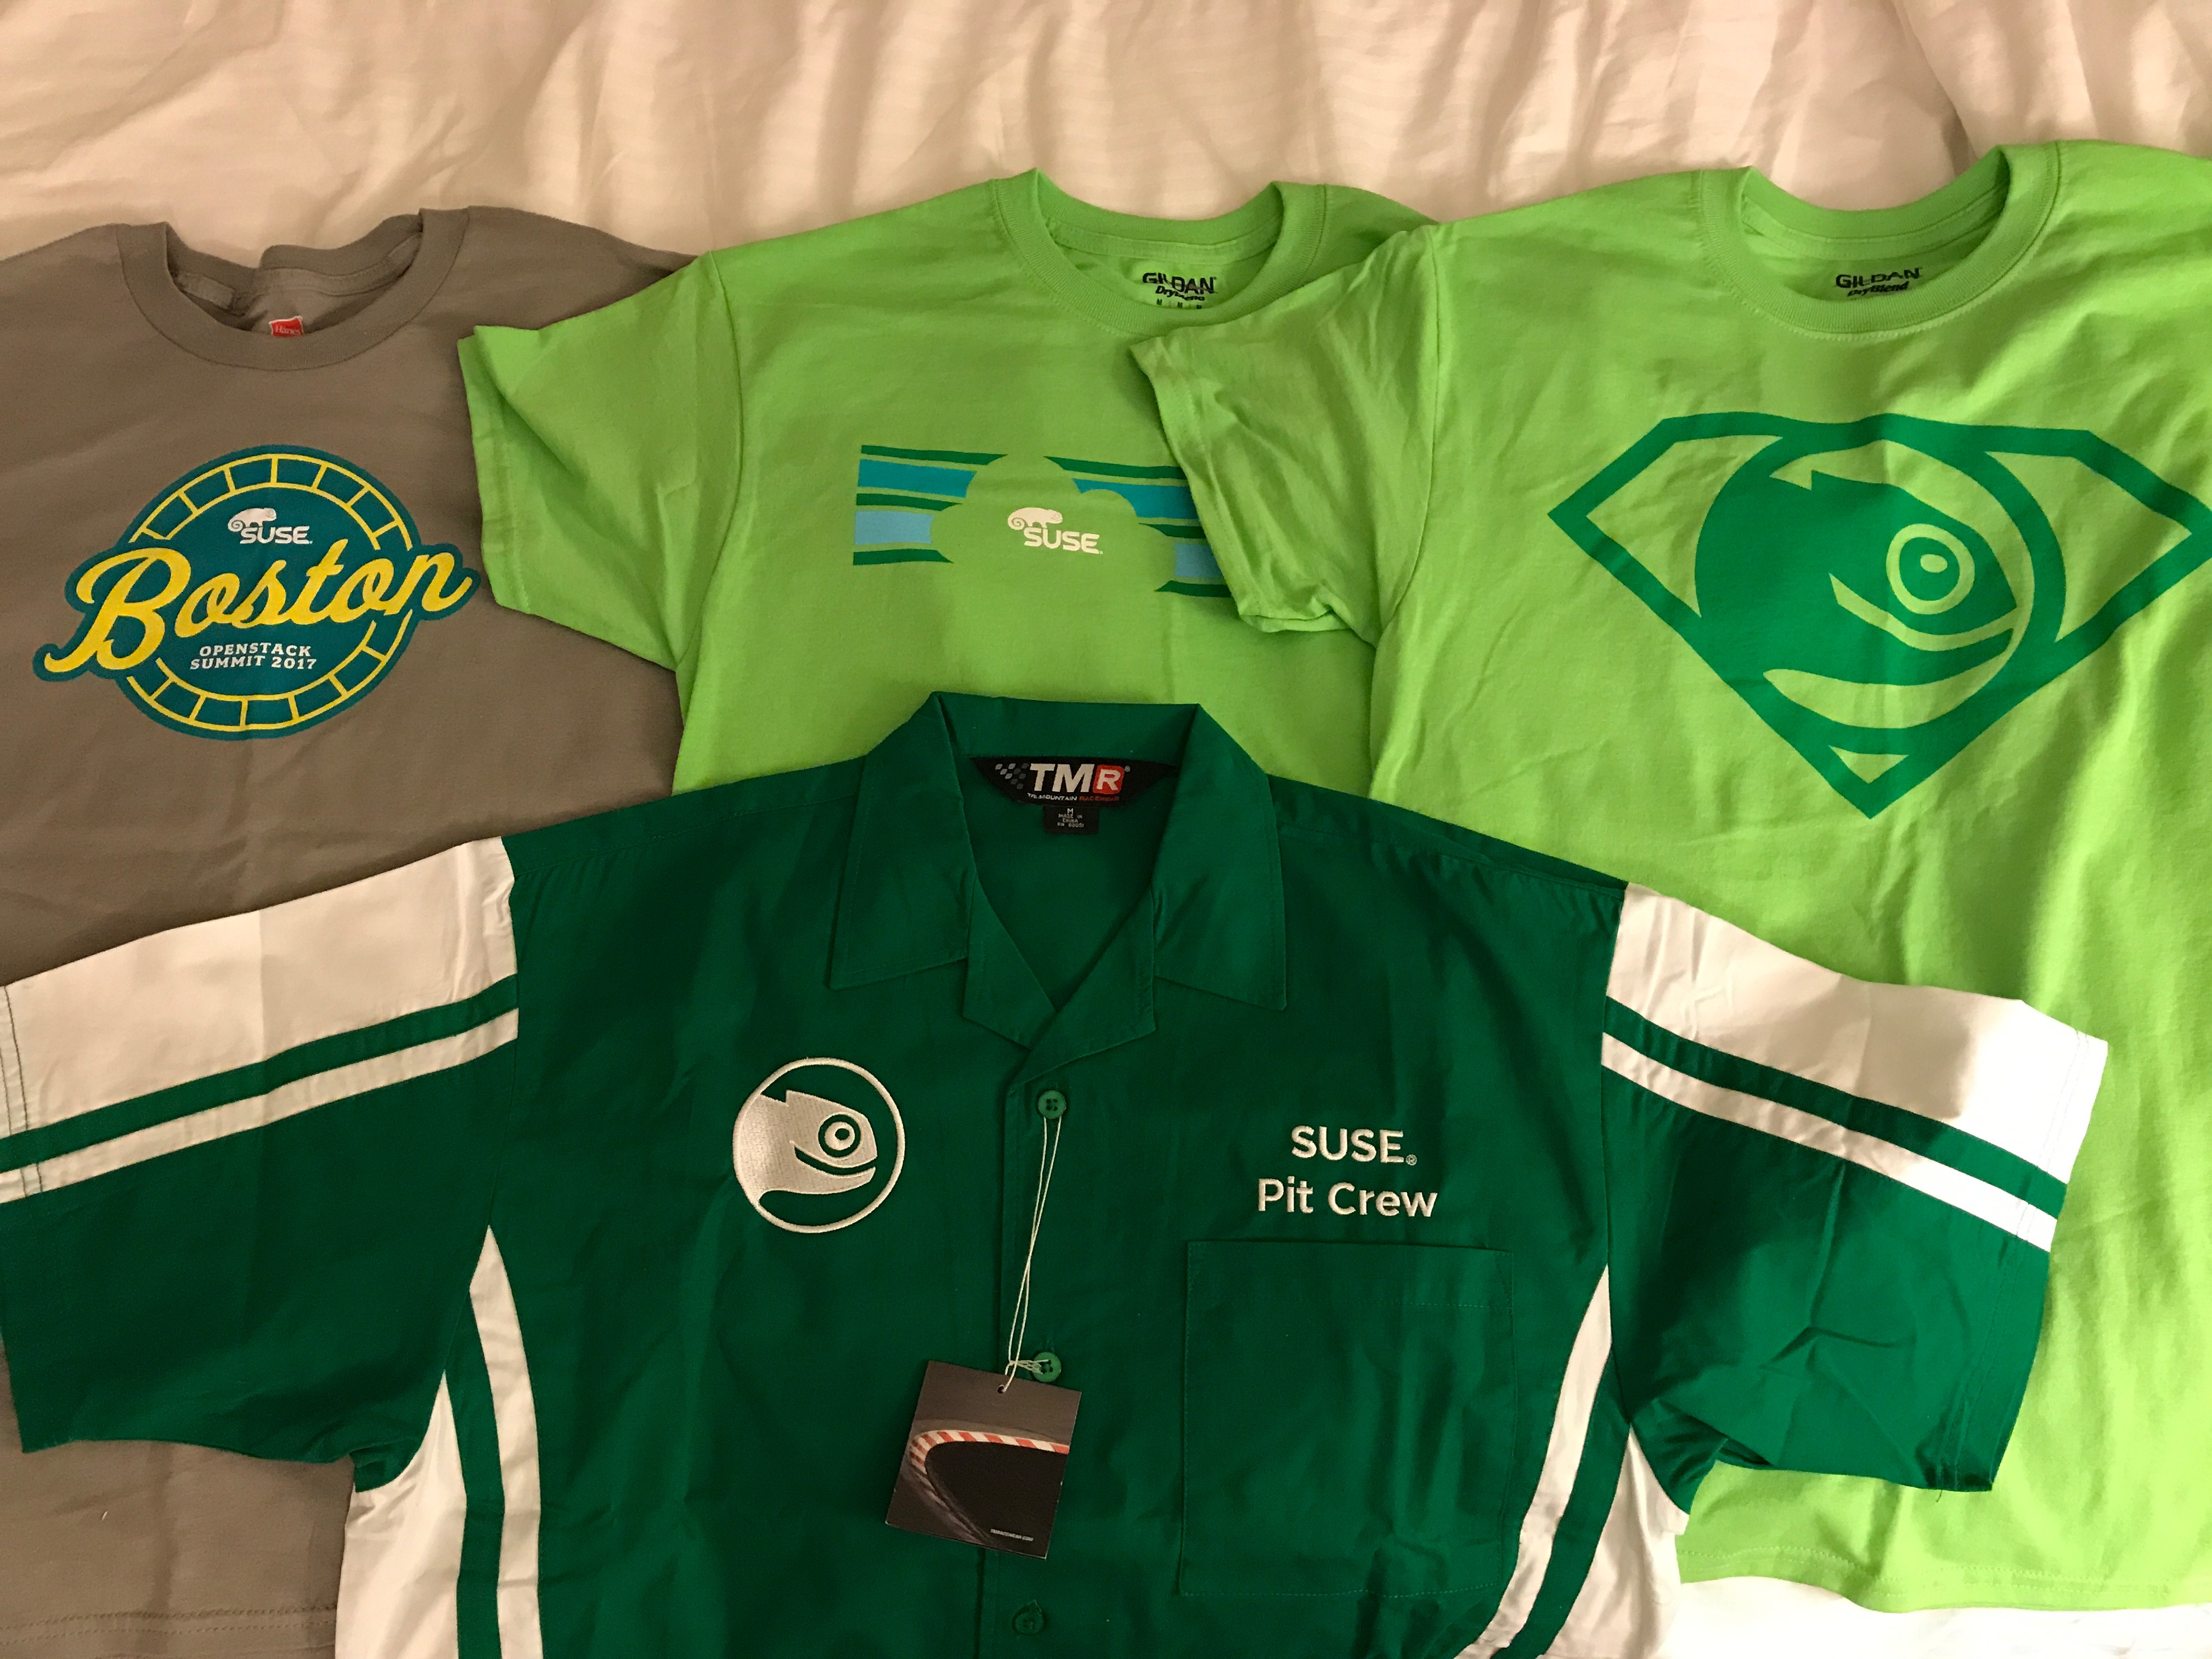
\includegraphics[width=1.0\textwidth]{suse-t-shirts.jpg}
    \end{column}
  \end{columns}
\end{frame}

\begin{frame}
  \frametitle{やりたいこと}
  \begin{columns}[T]
    \begin{column}{.5\textwidth}
      \begin{itemize}
        \item Mesos? DC/OS? なにそれ?
        \item[] (まずは)手元のマシンで使ってみたい!
        \item Mac → \href{https://ja.wikipedia.org/wiki/OpenSUSE}{openSUSE(Linux)}
          \begin{itemize}
            \item Dell Precision 5510 (Ubuntu pre-installed)
            \begin{itemize}
              \item[CPU:] Corei7@2.70GHz
              \item[Mem:] 32GB
              \item[HDD:] 500GB(SSD) + 1TB(HDD)
            \end{itemize}
          \end{itemize}
        \item Vagrant, OpenStack, etc.
      \end{itemize}
    \end{column}
    \begin{column}{.5\textwidth}
      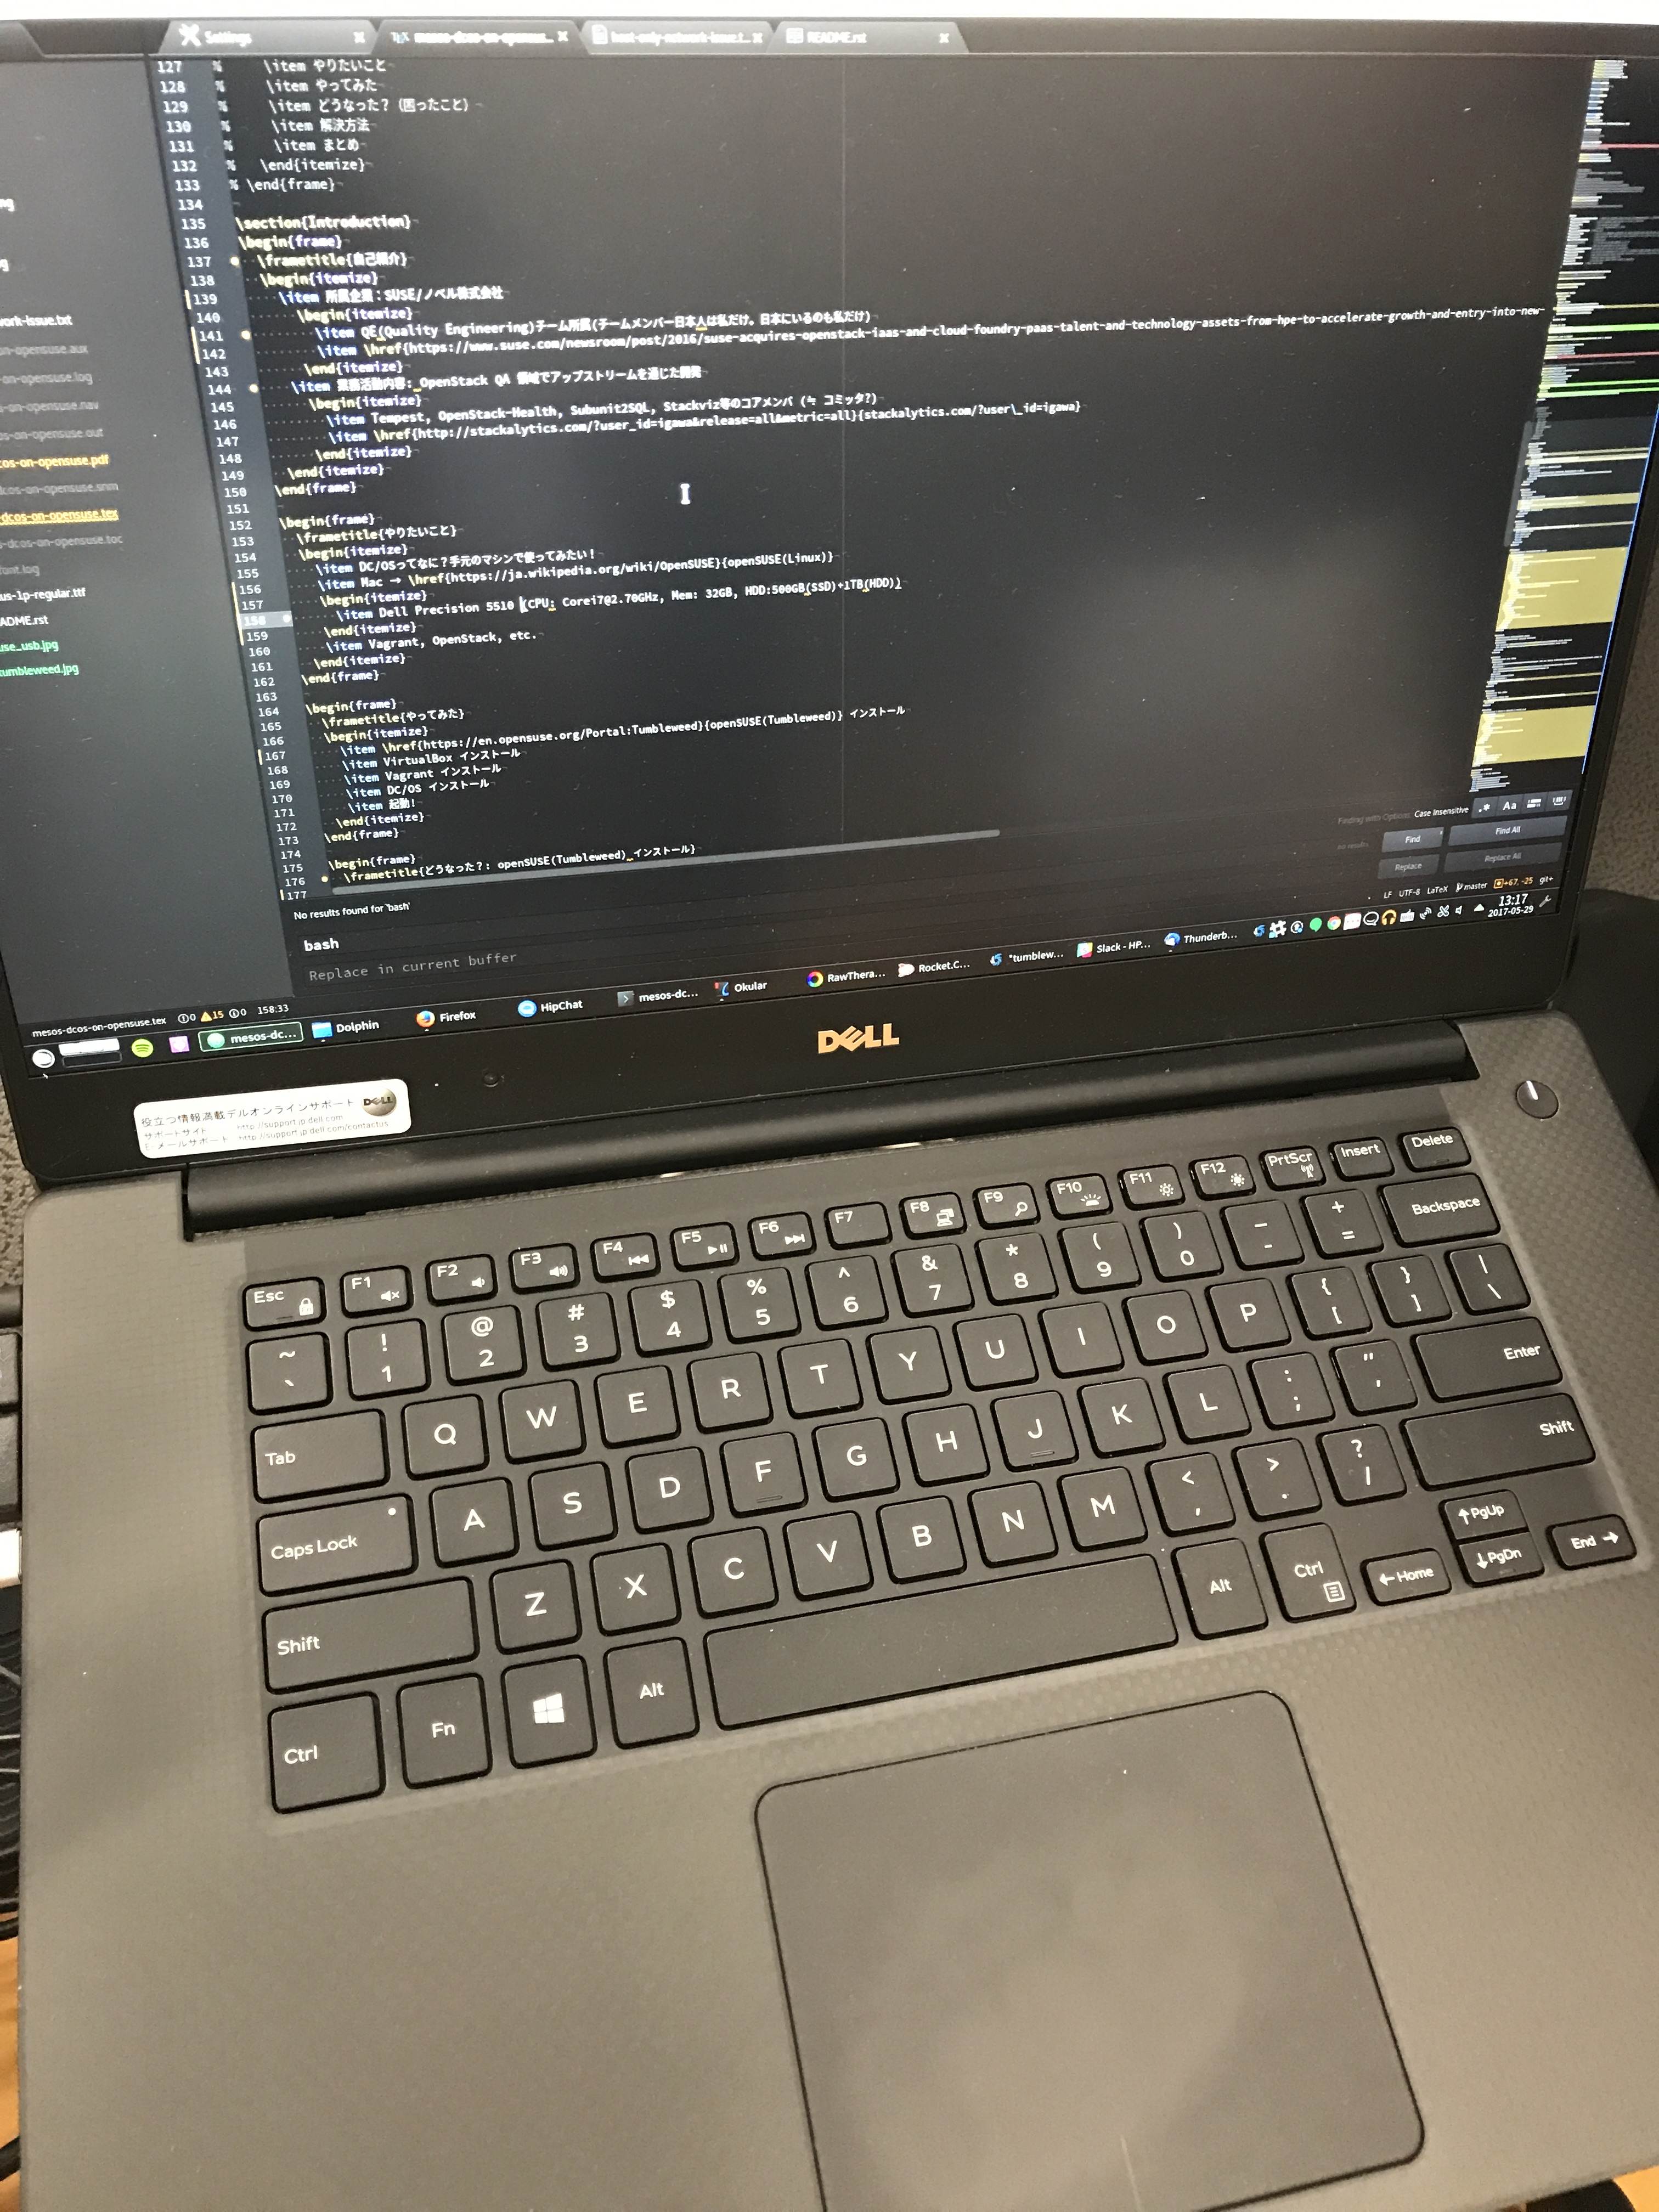
\includegraphics[height=1.1\textwidth]{dell_precision_5510.jpg}
    \end{column}
  \end{columns}
\end{frame}

\begin{frame}
  \frametitle{やってみた}
  \begin{itemize}
    \item \href{https://en.opensuse.org/Portal:Tumbleweed}{openSUSE(Tumbleweed)} インストール
    \item VirtualBox インストール
    \item Vagrant インストール
    \item Mesos, DC/OS インストール
    \item 起動!
  \end{itemize}
\end{frame}

\begin{frame}
  \frametitle{どうなった?: openSUSE(Tumbleweed) インストール}
  \begin{columns}[T]
    \begin{column}{.45\textwidth}
      \begin{itemize}
        \item \href{https://www.opensuse.org/}{openSUSE} \href{https://www.opensuse.org/\#Tumbleweed}{Tumbleweed} ?
        \item USB メモリなんて持ってない
        \item 容量足りない
        \item ブートしない
      \end{itemize}
    \end{column}
    \begin{column}{0.28\textwidth}
      \begin{figure}
        \begin{center}
          \caption{Tumbleweed? (Photo by \href{https://www.flickr.com/photos/jezarnold/}{jezarnold})}
          
\includegraphics[width=1.0\textwidth]{tumbleweed.jpg}
        \end{center}
        \begin{center}
          \caption{USEメモリ(4GB)}
          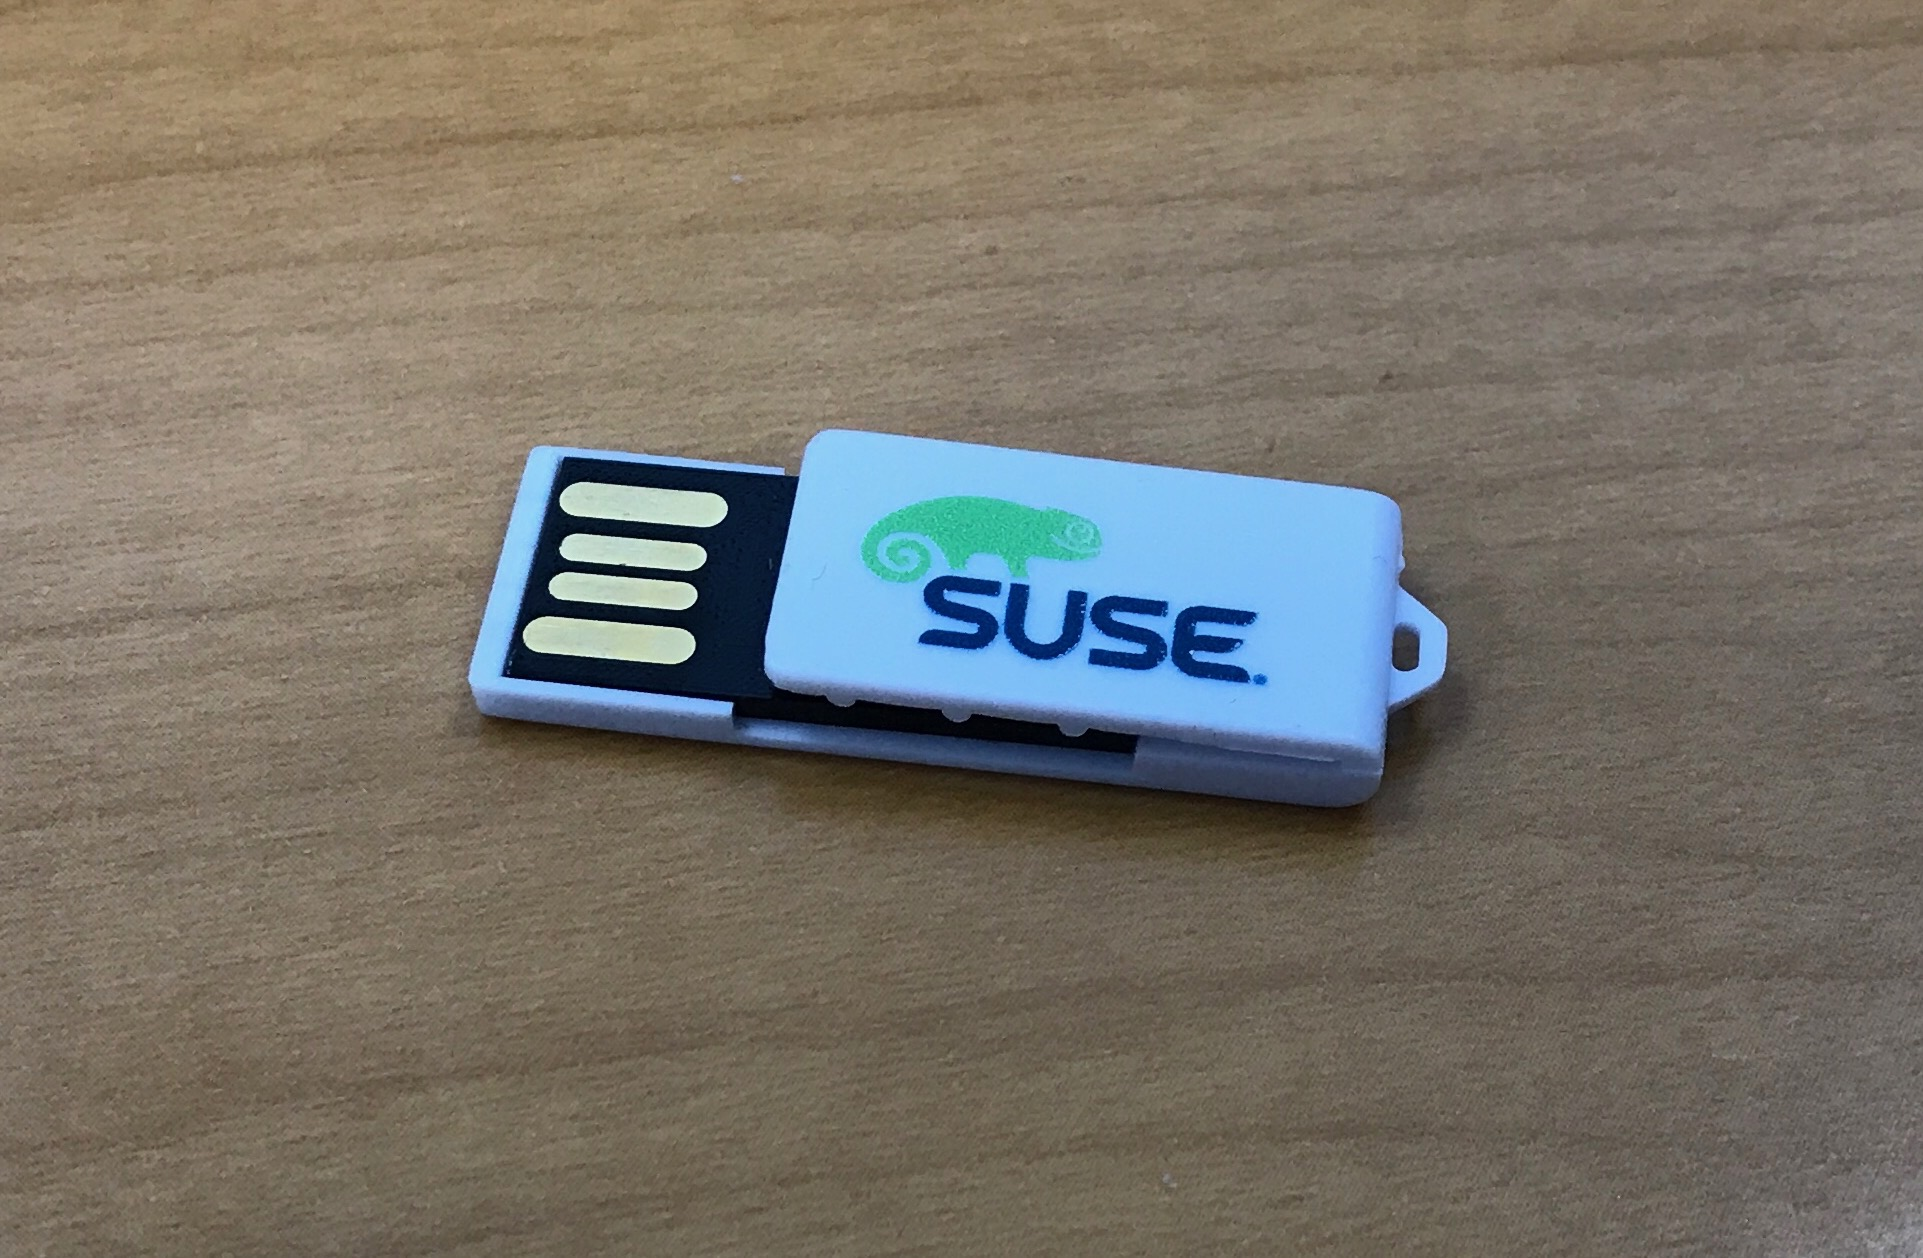
\includegraphics[width=1.0\textwidth]{suse_usb.jpg}
        \end{center}
      \end{figure}
    \end{column}
    \begin{column}{0.28\textwidth}
      \begin{figure}
        \begin{center}
          \caption{Boot error}
          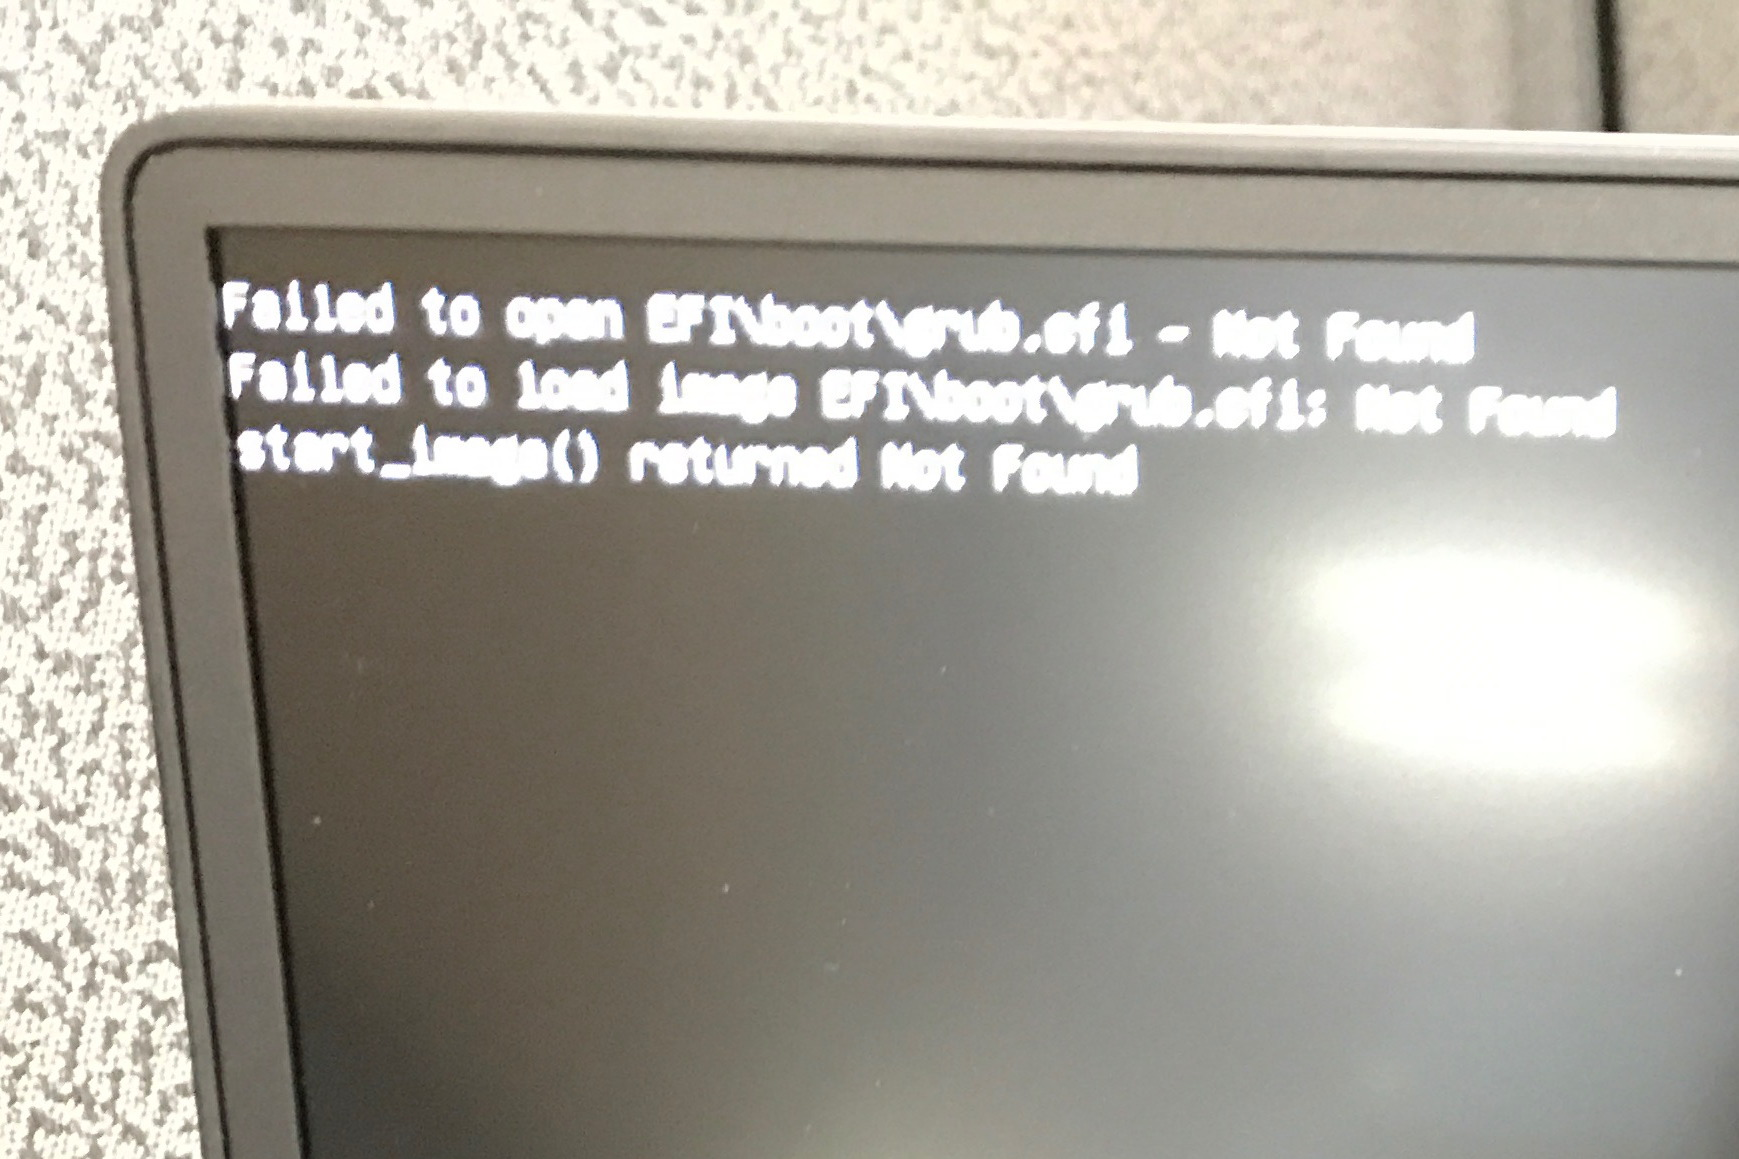
\includegraphics[width=1.0\textwidth]{boot.jpg}
        \end{center}
      \end{figure}
    \end{column}
  \end{columns}
\end{frame}

\begin{frame}
  \frametitle{どうなった?: VirtualBox/Vagrant インストール}
  それぞれの公式サイト(VirtualBox/Vagrant)に Tumbleweed 用のパッケージなし...
  \begin{itemize}
    \item VirtualBox: \lstinline[basicstyle=\ttfamily\footnotesize,columns=fixed]{zypper install virtualbox}
    \item Vagrant: \lstinline[basicstyle=\ttfamily\footnotesize,columns=fixed]{zypper install vagrant}
  \end{itemize}
\end{frame}

\begin{frame}
  \frametitle{どうなった?: DC/OS インストール}
  \begin{itemize}
    \item \href{https://dcos.io/docs/1.9/installing/local/}{Install DC/OS with Vagrant} に従い、\href{https://github.com/dcos/dcos-vagrant/}{master branch} を使用
    \begin{itemize}
      \item \lstinline[basicstyle=\ttfamily\footnotesize,columns=fixed]{cp VagrantConfig-1m-1a-1p.yaml VagrantConfig.yaml}
      \item \lstinline[basicstyle=\ttfamily\footnotesize,columns=fixed]{vagrant up}
    \end{itemize}
    \item すんなりインストールが進だ!4つのVMが起動した!
    \item 自動テスト(?)も通った!(っぽい)
    \item \url{http://m1.dcos} にアクセス! → つながらない・・ orz
  \end{itemize}
\end{frame}

\begin{frame}
  \frametitle{解決: DC/OS インストール}
  \begin{itemize}
    \item Host-only Networks issue
      \lstinputlisting[basicstyle=\ttfamily\footnotesize,frame=single,language=ruby]{host-only-network-issue.txt}
  \end{itemize}
\end{frame}

\begin{frame}
  \frametitle{DC/OS on Vagrant on VirtualBox on openSUSE 起動\!}
  \begin{columns}[T]
    \begin{column}{.50\textwidth}
      \begin{center}
        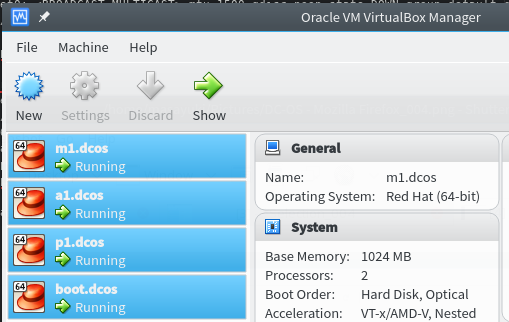
\includegraphics[width=1.0\textwidth]{dcos_vms.png}
      \end{center}
    \end{column}
    \begin{column}{.50\textwidth}
      \begin{center}
        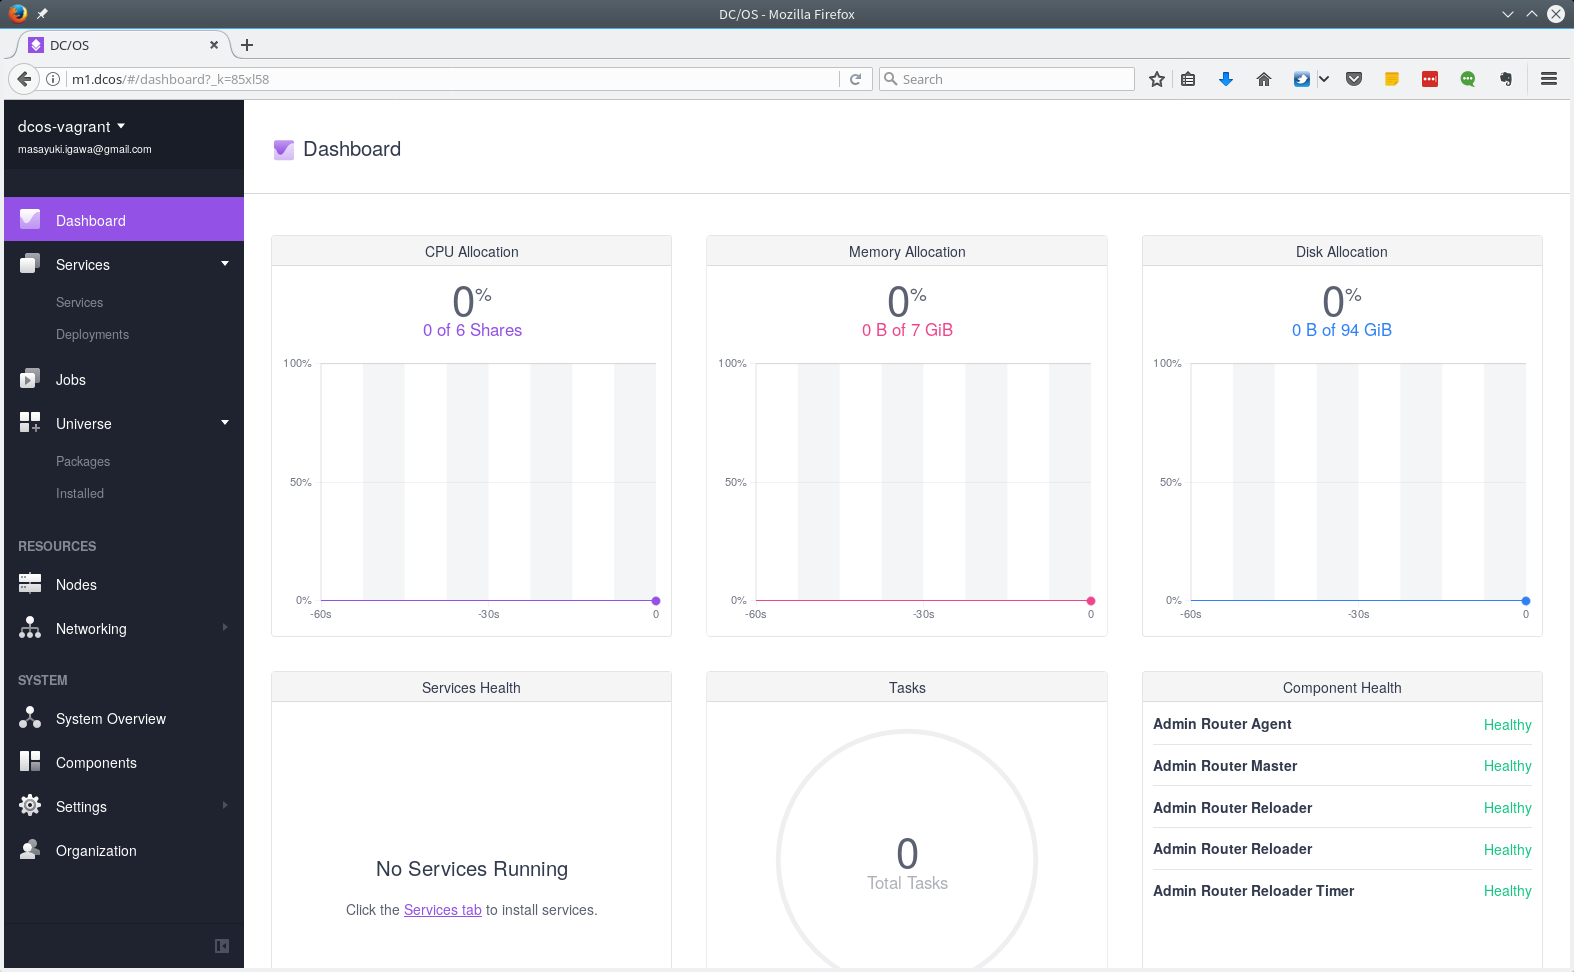
\includegraphics[width=1.0\textwidth]{DCOS_firefox.png}
      \end{center}
    \end{column}
  \end{columns}
\end{frame}

\subsection{Conclusion}
\begin{frame}
\frametitle{まとめ}
  \begin{itemize}
    \item openSUSE でも Mesos, DC/OS 使えるよ
    \item いろいろつまづくことがあるよ(Network...)
    \item 本番はこれから → 複数マシン・VMを管理したいよ
  \end{itemize}
\end{frame}

\subsection{More Information}
\begin{frame}
\frametitle{Where to get more information}
  \begin{itemize}
    \item \url{https://www.opensuse.org/\#Tumbleweed}
    \item \url{https://www.virtualbox.org/}
    \item \url{https://www.vagrantup.com/}
    \item \url{https://dcos.io/docs/1.9/installing/local/}
    \item \url{https://github.com/dcos/dcos-vagrant/}
  \end{itemize}
\end{frame}

\end{document}
